\documentclass[20pt, a4paper]{report}
\usepackage{graphicx}
\usepackage{amsmath}
\usepackage{mathtools}
%\usepackage{newtxtext,newtxmath}
\usepackage{hyperref}
\hypersetup{
	colorlinks=true,
	urlcolor=red,
	linkcolor=red,
}

\begin{document}


	\chapter{}
	\section{Non-linear Regression}
		\subsection{Polynomial Regression}
			\subsubsection{Brief Introduction}
			The aim of Polynomial regression is to find the best polynomial fit to a given set of points. The best fit depends on order of the polynomial. Higher order polynomials are more susceptible to noise and oscillate violently. A lower order polynomial gives better generalization, but may often fail to capture diversity in the curve.A good estimate usually tries to find a balance between the two.
			\linebreak \linebreak The polynomial regression model 
			\begin{align*}
			y_{i} &= \beta_{0}+\beta_{1}x_{i}+\beta_{2}x_{i}^{2}+\ldots+\beta_{m}x_{i}^{m}+\epsilon_{i} &(1,2,\ldots,n)
			\end{align*}
			can be expressed in matrix form as \begin{align*}
			{\displaystyle {\begin{bmatrix}y_{1}\\y_{2}\\y_{3}\\\vdots \\y_{n}\end{bmatrix}}={\begin{bmatrix}1&x_{1}&x_{1}^{2}&\dots &x_{1}^{m}\\1&x_{2}&x_{2}^{2}&\dots &x_{2}^{m}\\1&x_{3}&x_{3}^{2}&\dots &x_{3}^{m}\\\vdots &\vdots &\vdots &\ddots &\vdots \\1&x_{n}&x_{n}^{2}&\dots &x_{n}^{m}\end{bmatrix}}{\begin{bmatrix}\beta _{0}\\\beta _{1}\\\beta _{2}\\\vdots \\\beta _{m}\end{bmatrix}}+{\begin{bmatrix}\varepsilon _{1}\\\varepsilon _{2}\\\varepsilon _{3}\\\vdots \\\varepsilon _{n}\end{bmatrix}},}
			\end{align*}
			which when using pure matrix notation is written as

   $$ {\displaystyle {\vec {y}}=\mathbf {X} {\vec {\beta }}+{\vec {\varepsilon }}.\,} $$
   The polynomial regression can be expressed in terms of multiple linear regression with parameters $[1, x, x^{2}, \ldots,x^{n}]$, and hence, can be solved using least square optimization algorithms with $${\displaystyle {\widehat {\vec {\beta }}}=(\mathbf {X} ^{\mathsf {T}}\mathbf {X} )^{-1}\;\mathbf {X} ^{\mathsf {T}}{\vec {y}},\,}$$.
			\subsubsection{Polynomial used for fit}
			 For contactor tolerance curve, a 4th order polynomial of type $$y = a1 + a2*x + a_{3}*x^2 + a_{4}*x^3 +a_{5}*x^4$$. You can see the figure resulting from fit. 
			\begin{figure}[h]
%				\includegraphics[width=\textwidth]{contactor_fit.eps}
				\centering
			\end{figure}						
			The contactor curve fitting was done between $y$ and $x$, with $y$ as the independent variable. In other words, we fit a curve $x = f(y)$ instead of $ y = f(x) $.
		
		\subsection{Exponential regression}
		
		An alternate procedure,particularly for some contactor curves, is to use exponential regression, by fitting 
		$$ y(x) = \beta_{0}e^{\beta_{1}x}$$.We then try to estimate the parameters $\beta_{0}$ and $\beta_{1}$ subject to given vector points $Y^{T}$ and $X^{T}$ by minimizing the objective function $$ \phi = \frac{1}{2}\sum_{i=1}^{n}(\beta_{0}e^{\beta_{1}x_{i}}-y_{i})^{2}.$$ subject to the given vector points 
		\begin{align*}
		Y^{T} = (y_{1},y_{2},\ldots,y_{n})\\
		X^{T} = (x_{1},x_{2},\ldots,x_{n})\\
	\end{align*}	  	
		Exponential regression is useful for contactor curves with phase shifts of $(0^{0},\ldots,20^{0})$.
		
		\subsection{Step Regression}
		A step regression aims to fit a modified step function to the given data points. The modified step function can be formulated as \begin{align*}
		y = \begin{dcases}
					0,& x<=x_{base}\\
					y_{base},& x>x_{base}
				\end{dcases}
\end{align*}	
	where $x_{base}$ and $y_{base}$ are the threshold values for the independent and dependent variables $x$ and $y$ respectively. 
	 A least-squares fit usually gives a very poor estimate of the function, as it contains a large number of local minima. To fix this , usually it is necessary to initialize the threshold values to near optimal values. 
	 Consequently, it is used only with rectangular sag curves. 	 
		
		\section{Levenberg-Marquardt Algorithm}
		
		\subsection{The problem statement}
		
		The primary application of the Levenberg–Marquardt algorithm is in the least-squares curve fitting problem; given a set of m points $(x_{i}, y_{i})$, determine the parameters $\beta$ to the model curve $f(x,\beta)$, so that the sum of squares of deviations is minimized.
		$${\displaystyle {\hat {\beta }}=\operatorname*{argmin} \limits _{\beta }S(\beta )\equiv \operatorname {argmin} \limits _{\beta }\sum _{i=1}^{m}[y_{i}-f(x_{i},{\boldsymbol {\beta }})]^{2}.}$$
		\subsection{Solution}
		Like other numeric minimization algorithms, the Levenberg–Marquardt algorithm is an iterative procedure. To start a minimization, the user has to provide an initial guess for the parameter vector, $\beta$. In cases with only one minimum, an uninformed standard guess like $\beta^{T} = (1, 1,\ldots, 1)$ will work fine; in cases with multiple minima, the algorithm converges to the global minimum only if the initial guess is already somewhat close to the final solution.
		
		 In each iteration step, the parameter vector $\beta$ is replaced by a new estimate $\beta + \delta$. To determine $\delta$, the function $f ( x_{i} , \beta + \delta )$ $${\displaystyle f(x_{i},{\boldsymbol {\beta }}+{\boldsymbol {\delta }})}$$ is approximated by its linearization: $${\displaystyle f(x_{i},{\boldsymbol {\beta }}+{\boldsymbol {\delta }})\approx f(x_{i},{\boldsymbol {\beta }})+J_{i}{\boldsymbol {\delta }},}$$
		 where $${\displaystyle J_{i}={\frac {\partial f(x_{i},{\boldsymbol {\beta }})}{\partial {\boldsymbol {\beta }}}}}$$.
		 
		 is the gradient (row-vector in this case) of $f$ with respect to $\beta$.
		 The sum $S(\beta)$ has it's minimum at zero gradient with respect to $\beta$. The first order approximation of $f(x_{i},\beta+\delta)$ is given by:\begin{equation*}
		 {\displaystyle S({\boldsymbol {\beta }}+{\boldsymbol {\delta }})\approx \sum _{i=1}^{m}\left(y_{i}-f(x_{i},{\boldsymbol {\beta }})-J_{i}{\boldsymbol {\delta }}\right)^{2},}
\end{equation*}		  
	Or in vector notation,\begin{equation*}
	{\displaystyle {\begin{aligned}S({\boldsymbol {\beta }}+{\boldsymbol {\delta }})&\approx [\mathbf {y} -\mathbf {f} ({\boldsymbol {\beta }})]^{T}[\mathbf {y} -\mathbf {f} ({\boldsymbol {\beta }})]-2[\mathbf {y} -\mathbf {f} ({\boldsymbol {\beta }})]^{T}\mathbf {J} {\boldsymbol {\delta }}+{\boldsymbol {\delta }}^{T}\mathbf {J} ^{T}\mathbf {J} {\boldsymbol {\delta }}.\end{aligned}}}
	\end{equation*}
	Taking the derivative of $S(\beta+\delta)$ with respect to $\delta$ and setting the result to zero yields \begin{align*}
	{\displaystyle (\mathbf {J} ^{T}\mathbf {J} ){\boldsymbol {\delta }}=\mathbf {J} ^{T}[\mathbf {y} -f({\boldsymbol {\beta }})],}
\end{align*}
	
	Or as a damped version, \begin{align*}
	{\displaystyle (\mathbf {J} ^{T}\mathbf {J} +\lambda \mathbf {I} ){\boldsymbol {\delta }}=\mathbf {J} ^{T}[\mathbf {y} -\mathbf {f} ({\boldsymbol {\beta }})],}
\end{align*}	
Marquardt proposed an alternative modification to Levenberg's method to avoid slow convergence with large damping factor $\lambda$ as,
\begin{align*}
{\displaystyle [\mathbf {J} ^{T}\mathbf {J} +\lambda \operatorname {diag} (\mathbf {J} ^{T}\mathbf {J} )]{\boldsymbol {\delta }}=\mathbf {J} ^{T}[\mathbf {y} -\mathbf {f} ({\boldsymbol {\beta }})].}
\end{align*}

	The value of damping factor $\lambda$ is decreased or increased per iteration as follows:
	\begin{enumerate}
	\item Choose initial parameters $\lambda_{i}$ and reduction parameter $\nu$. The are usually drawn randomly from normal distribution. 
	\item Perform a step $S(\beta)$ with $\lambda_{i}$ and check if $S(\beta)$ has reduced.
	\item Now decrease $\lambda_{i}$ as $\frac{\lambda_{i} }{\nu}$, and evaluate $S(\beta)$. 
	\item If a reduction is observed in $S(\beta)$, use the new value of $\lambda = \frac{\lambda_{i} }{\nu}$.
	\item If step(3) doesn't produce good enough results, then multiply $\lambda_{i}$ with $\nu$ and evaluate $S(\beta)$ again. If a reduction is observed, update $\lambda$ as $lambda = \lambda_{i}*\nu$
	\item Perform steps $(2\ldots 5)$ until minima is reached.
\end{enumerate}	
	 
		For more information refer Wikipedia page at \href{https://en.wikipedia.org/wiki/Levenberg%E2%80%93Marquardt_algorithm}{Levenberg-Marquardt Algorithm}
			
			\section{Trip calculations}
			\subsection{Rectangular Sag curves}
			For Rectangular sag curves, two methods has been formulated. \begin{enumerate}
				\item In this method, the points are assigned uniform probability through $\tanh$ operator. The sag points $(x_{sag}, y_{sag})$ are compared, and origin shifted with respect to $(x_{tolerance},y_{tolerance})$. 
				The probability is then assigned as 
				\begin{equation*}
					probability = \tanh((y_{sag}-y_{min})*(y_{max}-y_{sag})) * \tanh((x_{sag}-x_{min})*(x_{max}-x_{sag}))
				\end{equation*}
				But it gives false positives for region$$x_{min} \leq x_{sag} \leq x_{max}$$.
				To mitigate this $2^{nd}$ procedure is proposed.
				\item This method works by dividing the tolerance curves into multiple areas, as shown in \ref{fig:rec_tol}.
				\begin{figure}[!h]
				\centering
%			\includegraphics[scale=0.3]{rect_tol}	
			\caption{Rectangular Tolerance curve showing different areas of possible trip}
			\label{fig:rec_tol}
\end{figure}. 
\paragraph{}In region I and V, the equipment trip is certain, with probability of 0 and 1 for trip respectively.

\begin{figure}[!h]
\centering
%\includegraphics[scale=0.5]{Rect_point1}
\caption{A typical sag point on region III}
\end{figure}
\begin{table}
	\begin{tabular}{|c|c|}
	\hline
	Region& Trip Status \\ \hline
	I & Won't trip\\
	\hline
	II & May trip depending on voltage sag severity\\ \hline
	III & May trip, depending on both voltage severity and duration\\ \hline
	IV & May trip depending upon duration \\ \hline
	V & Will trip \\
	\hline
	
	\end{tabular}
	\caption{Summary of trip by region}
	\label{tab:trip_summary}
	\end{table}
	\newpage Regions II, IV and III are uncertain. \textbf{Our first contribution} is a method for determining the probability of trip in the regions. In region II, the probability depends on voltage sag only, whereas in region IV it depends on duration entirely. In region III, it depends on both. It is summarized in table \ref{tab:trip_summary}
	
 A uniform exponential probability distribution is assigned to them, as per equations below: 								
				 
				\begin{equation*}
					y = \begin{dcases}
					0, {x_{sag} \leq x_{min} , y_{sag} \geq y_{min}}\\
					e^{\ln(2)*(x_{sag}-x_{min})/(x_{max}-x_{min}))-1}, 	x_{min} \leq x_{sag} \leq x_{max}, y_{sag} \leq y_{min}\\			
					e^{\ln(2)*(y_{sag}-y_{max})/(y_{min}-y_{max}))-1}, 	x_{sag} \geq x_{max},  y_{sag} \geq y_{max}\\
					1, x_{max} \leq x_{sag}, y_{sag} \leq y_{max}\\		
					\end{dcases}
				\end{equation*}
				\linebreak Else 
				\begin{equation*}
					y = e^{\ln(2)*(x_{sag}-x_{min})/(x_{max}-x_{min}))-1}*e^{\ln(2)*(y_{sag}-y_{max})/(y_{min}-y_{max}))-1}
				\end{equation*}
				If , 	\begin{equation*}
				x_{min} \leq x_{sag} \leq x_{max} , y_{min} \geq y_{sag} \geq y_{max}
				\end{equation*}
				This region-wise division gives a better estimate of trip probability.
				
			\end{enumerate}
			
			\subsection{Contactor sag curves}
			\begin{figure}[!h]
			\centering
			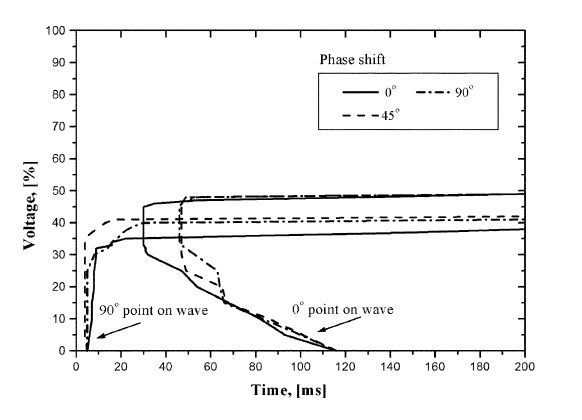
\includegraphics[scale=0.6]{contactor}
			\caption{Typical Contactor curves}
			\label{Contactor_curves}
			\end{figure}
			 For contactor Tolerance Curves, the probability is calculated by two methods as follows:
			 
			  \paragraph{Method 1:} The probability is calculated by taking Pseudo inverse. It is therefore, ideal for $90_{o}$ point on curve only.
			 \paragraph{Algorithm:}
			 \begin{enumerate}
			 \item Fit polynomial curve $y = f(x)$.
			 \item get a sag point $(x_{sag}, y_{sag})$
			 \item Determine corresponding values $(x_{f},y_{f})$ from fitted curve as $$ y_{f} = f(x_{sag})$$
			 $$x_{f} = (b^{T}*b)^{-1}*b^{T}*y$$.
			 Here, we have taken the Moore-Penrose Pseudo inverse to determine $x_{f}$.
			 \item Calculate probability as 
			 \begin{equation*}
			 	y = \begin{dcases}
			 	0,& x_{sag} \leq x_{f}, y_{sag} \geq y_{f}\\
			 	\tanh(\eta*(x_{f}-x_{sag})*(y_{f}-y_{sag})),&otherwise\\
			 	\end{dcases}
\end{equation*}		
		Where $\eta$ is a parameter used to control probability steepness.	  
			 \end{enumerate}
			   \paragraph{Method 2:} The probability is calculated by estimating parameters with numerical methods or simulated annealing. The algorithm works moderately well with $0_{o}$ point on curve, and well with $90_{o}$ point on curve. 
			 \paragraph{Algorithm:}
			 \begin{enumerate}
			 \item Fit polynomial curve $y = f(x)$.
			 \item get a sag point $(x_{sag}, y_{sag})$
			 \item Determine corresponding values $(x_{f},y_{f})$ from fitted curve as $$ y_{f} = f(x_{sag})$$
			 $x_{f}$ can only be calculated by minimizing least squares error 
			 $$\sum_{i=0}^{n}(f(y)-y_{sag})^{2}$$
			 by numerical methods, or simulated annealing, to find $x_{f}$, which will minimize the given error function. We used simulated annealing.
			 \item Calculate probability as 
			 \begin{equation*}
			 	y = \begin{dcases}
			 	0,& x_{sag} \leq x_{f}, y_{sag} \geq y_{f}\\
			 	\tanh(\eta*(x_{f}-x_{sag})*(y_{f}-y_{sag})),&otherwise\\
			 	\end{dcases}
\end{equation*}		
		Where $\eta$ is a parameter used to control probability steepness.	
		\end{enumerate}
		
		\paragraph{Caveats:}The process is not error free, especially for $0_{o}$ point on curve. We are working on a cubic spline interpolation method, which gives better results. 
			
			\subsection{Process Trip}
			Let us assume two machines with probability of trip $p_{1}$ and $p_{2}$ are connected in \begin{enumerate}
			\item{Series:} Process probability is $$ y = \max{(p_{1}, p_{2})}$$ 
			\item{Parallel:} Process probability is $$ y = \min{(p_{1}, p_{2})}$$
			\end{enumerate}
			
			For multiple series parallel machines, stack up the probabilities in cascade as per above rules. The individual probabilities can be easily determined as well.		
		
	
\end{document}